% ------------------------------------------------------------------------
% Template zur Erstellung von Seminararbeiten am Lehrstuhl für Wirtschaftsinformatik I
% der Universität Stuttgart
%
% Erstellerin: Jella Pfeiffer (08.10.2019)
% Überarbeitet von: Pascal Heßler, Paul Herbst
% weiter überarbeitet von: Paul Herbst (paul.herbst@bwi.uni-stuttgart.de) am 08.05.2024
% zuletzt überarbeitet von: Philipp Burow (philipp.burow@bwi-uni-stuttgart.de) am 20.02.2025
%
% Bitte auch die README.md beachten!
% ------------------------------------------------------------------------

% ------------------------------------------------------------------------
% Allgemeine Einstellungen
% ------------------------------------------------------------------------
\documentclass[12pt]{article}
\usepackage[paper=a4paper,left=25mm,right=25mm,top=25mm,bottom=20mm]{geometry}
\usepackage[utf8]{inputenc}       % Auskommentiert lassen wenn LuaLaTeX verwendet wird, nur relevant für pdfLaTeX
\usepackage[english]{babel}       % Verwende deutsche, bzw. amerikanische Silbentrennung
\usepackage[ngerman]{babel}         % Deutsche Alternative
\usepackage{setspace}               
\usepackage{fontspec}
\setlength{\parindent}{0pt}         % Setzt den Einzug von neuen Paragraphen auf 0
\setlength{\parskip}{1.2ex}         % setzt den Abstand zwischen zwei Paragraphen auf 1.2
\setmainfont{Arial}

% ------------------------------------------------------------------------
% Literatur
% ------------------------------------------------------------------------
% Achtung zur Einbindung der Literatur wird hier Biber verwendet und nich der Standard BibTex. In Sublime muss nichts verändert werden.
% 1. Sicherstellen, dass Biber installiert ist ->  in Tex Live vorinstalliert
% 2. Stellt eure Schreibumgebung um -> In TeXstudio: Optionen -> TeXstudio konfigurieren -> Erzeugen -> Standard Bibliographieprogramm
\usepackage[backend=biber,style=apa,natbib=false]{biblatex}
\DeclareLanguageMapping{american}{american-apa}         % Sprach Einstellung
\addbibresource{literature.bib}       % Legt die Datei fest in der die Literatur liegt (z. B.: Export aus Citavi)
\usepackage{breakcites}                                 % Falls Zitationen nicht ans Zeilenende passen
\usepackage{csquotes}                                   % Erweitert die Möglichkeiten beim zitieren

% ------------------------------------------------------------------------
% Mathematische Symbole
% ------------------------------------------------------------------------
\usepackage{amssymb}
\usepackage{amsmath}        % Formattierung von Tabellen und Matritzen

% ------------------------------------------------------------------------
% Beschriftungen
% ------------------------------------------------------------------------
\usepackage{caption}   
\captionsetup[figure]{font={small, it}, belowskip=4pt}
\captionsetup[table]{font={small, it}, belowskip=4pt}

% ------------------------------------------------------------------------
% Grafiken
% ------------------------------------------------------------------------
\usepackage{graphicx}       % Zum Einbinden von Grafiken
\usepackage{subfigure}      % Um Bilder innerhalb einer Figure anzuordnen (Bild a b c d...)

% ------------------------------------------------------------------------
% Tabellen
% Um einfache Tabellen zu erstellen kann https://www.tablesgenerator.com/ verwendet werden.
% ------------------------------------------------------------------------
\usepackage{tabularx}       % Ermöglicht weitere Tabellen Einstellungen
\usepackage{multirow}       % Ermöglicht Zellen zu verbinden
\usepackage{booktabs}       % Tabellen Midline Topline etc.
\usepackage{float}          % Tabelen Positionierung
\usepackage{longtable}      % Ermöglicht Tabellen über mehrere Seiten hinweg, so dass sie noch dasselbe Format besitzten ftp://ftp.fu-berlin.de/tex/CTAN/macros/latex/required/tools/longtable.pdf


% ------------------------------------------------------------------------
% Überschriften Formatierung
% ------------------------------------------------------------------------
\usepackage{titlesec}       % Ermöglicht die Formatierung von Überschriften
% Schriftgröße, Schriftart und Abstand
\titleformat{\section}{\normalfont\large\bfseries}{\thesection}{1em}{}
\titleformat{\subsection}{\normalfont\normalsize\bfseries}{\thesubsection}{1em}{}
\titleformat{\subsubsection}{\normalfont\normalsize\bfseries}{\thesubsubsection}{1em}{}
\titlespacing*{\section}{0pt}{1ex plus 0.5ex minus .2ex}{-0.5ex}
\titlespacing*{\subsection}{0pt}{0pt}{-6pt}
\titlespacing*{\subsubsection}{0pt}{0pt}{-6pt}
\renewcommand{\thesection}{\arabic{section}.}  
\renewcommand{\thesubsection}{\thesection\arabic{subsection}.}   
\renewcommand{\thesubsubsection}{\thesubsection\arabic{subsubsection}.}  

% ------------------------------------------------------------------------
% Kopf- und Fußzeile
% ------------------------------------------------------------------------
\usepackage{fancyhdr}       % Ermöglicht die Formatierung von Kopf- und Fußzeilen
\pagestyle{fancy}           % Setzt den Seitenstil auf fancy
\fancyhf{}                  % Löscht alle Kopf- und Fußzeilen
\fancyhead[R]{\thepage}     % Setzt die Seitenzahl auf der rechten Seite
\renewcommand{\headrulewidth}{0pt} % Entfernt die Linie unter der Kopfzeile
\renewcommand{\footrulewidth}{0pt} % Entfernt die Linie über der Fußzeile
\setlength{\headheight}{14.5pt}
\addtolength{\topmargin}{-2.5pt}

% ------------------------------------------------------------------------
% Inhaltsverzeichnis
% ------------------------------------------------------------------------
\makeatletter
\renewcommand{\l@figure}[2]{\@dottedtocline{1}{0em}{1.5em}{Abbildung~#1}{#2}} % Setzt Abbildung ins Abbildungsverzeichnis
\renewcommand{\l@table}[2]{\@dottedtocline{1}{0em}{1.5em}{Tabelle~#1}{#2}} % Setzt Tabelle ins Tabellenverzeichnis
\makeatother

% ------------------------------------------------------------------------
% Abkürzungen und Glossar
% VERWENDUNG: Hier die Abkürzungen definieren und im Text verwenden mit \gls{AI} oder \glspl{AI} für Plural
% Zur Aktualisierung "makeglossaries" bzw. "makeglossaries master" ausführen und dann nochmal kompilieren
% ------------------------------------------------------------------------
\usepackage[acronym,toc,nonumberlist]{glossaries} % Ermöglicht die Verwendung von Abkürzungen und Glossar

\makeglossaries

\newacronym{ai}{AI}{Artificial Intelligence}        % Hier werden die Abkürzungen definiert
\newacronym{ml}{ML}{Machine Learning}
\newacronym{nlp}{NLP}{Natural Language Processing}
\newacronym{ca}{CA}{Combinatorial Auctions}

% **********************************************************************************************************************
% Folgende Pakete sind rein optional und etwas komplexer in ihrer Umsetzung nur für etwas erfahrenere LaTeX User
% **********************************************************************************************************************
% \usepackage{siunitx}      % Ausrichten von Tabellen an dezimalstellen (Umsetzung etwas komplizierter)
% \usepackage{rccol}        % Ein Neues Format R (wird wahrscheinlich mit dem Folgenden R zu Problemen führen) und sorgt, dass nach , ausgerichtet wird und automatisches runden in Tabellen wird ermöglicht
% \usepackage{fltpoint}     % Gehört zu rccol
% \usepackage{dcolumn}      % Gehört zu rccol
%
% \newcolumntype{L}[1]{>{\raggedright\arraybackslash}p{#1}}       % Linksbündig mit Breitenangabe
% \newcolumntype{C}[1]{>{\centering\arraybackslash}p{#1}}         % Zentriert mit Breitenangabe
% \newcolumntype{R}[1]{>{\raggedleft\arraybackslash}p{#1}}        % Rechtsbündig mit Breitenangabe
% \newcolumntype{x}[1]{!{\centering\arraybackslash\vrule width #1}}

% ------------------------------------------------------------------------
% Sonstige
% ------------------------------------------------------------------------
\usepackage{scrhack}        % Löst unnötige Warnungen!
\usepackage{color}          % Ermöglicht Text einzufärben \pagecolor{FARBE}  \color{FARBE} \textcolor{FARBE}{TEXT} \colorbox{FARBE}{TEXT}
\usepackage{hyperref}       % Ermöglicht URLS schreibweise ist z.B. \url{http://www.uni-giessen.de}

\usepackage{eurosym}        % Für Euro Symbol \euro{} oder \eruo (Unterschieden sich bezüglich Leerzeichen danach)

\usepackage{framed}         % Einrahmen von Texten mit der shaded-Umgebung.

\usepackage{pdflscape}      % Querformat möglich über \begin{landscape} \end{landscape}

% ------------------------------------------------------------------------
% Fein Justierungen
% ------------------------------------------------------------------------
\DeclareMathOperator*{\argmax}{arg\,max}

\newenvironment{packed_enum}{
\begin{enumerate}
  \setlength{\itemsep}{1pt}
  \setlength{\parskip}{0pt}
  \setlength{\parsep}{0pt}
}{\end{enumerate}}

\hypersetup{hidelinks}                 % Versteckt die Links im PDF (optisch)

% ----- ende der präambel ----------------------------------
% Start des Dokuments
% ----------------------------------------------------------
\begin{document} 
% Theoretisch kann man auch alles in einem Dokument haben. Das ist jedoch unübersichtlich. Daher werden hier die einzelnen Kapitel eingebunden.
\pagenumbering{Alph}                  % Löst unnötigen Warnungen

%!TEX root = ../master.tex
% Die Titelseite der Arbeit

\begin{titlepage}
  % Vertikaler Zwischenraum
  \vspace*{5cm}

  % Titel der Arbeit und Typ der Arbeit, umrandet

  \begin{spacing}{1.5}

    \begin{center}
      {\large \textsc{THEMA 02:\\[7pt]}} % No need for double backslashes here
      {\large \textsc{Informationsbeschaffung und -konsolidierung mit LLM-basierten Multiagentensystemen}} % Kept large and textsc for each line

      \vspace*{1.5cm} 
      Seminararbeit im Rahmen des Seminars Wirtschaftsinformatik 1\\[6pt]
      im 2. Mastersemester
    \end{center}
  \end{spacing}

  \vfill


  \noindent
  \renewcommand{\arraystretch}{1.5} 

  % Daten des Erstellers, Einreichungsdatum in einer Tabelle ausgerichtet
  \begin{tabular*}{0.62\textwidth}{l@{\hspace{20pt}}l}
    vorgelegt bei: & Dr. Gero Strobel und Dr. Henning Baars \\
                   & Betriebswirtschaftl. Institut \\
                   & Abteilung VII, Wirtschaftsinformatik 1 \\[1cm]% Removed extra backslashes 

    Betreuer:      & Dr. Gero Strobel \\[1cm] % Removed extra backslashes

    von:           & Thomas Schaffrath \\
                   & Wildensteinstraße 21 70469 Stuttgart \\
                   & Studiengang: Wirtschaftsinformatik \\
                   & 353309 \\
  \end{tabular*}
  \vspace*{3cm}

\end{titlepage} % Ende des Titelblatts

              % Titelseite einbinden

\pagenumbering{Roman}                 % Löst unnötigen Warnungen
\setcounter{page}{2}                  % setzt die Seitenzahl auf 2

% ------------------------------------------------------------------------
% Verzeichnisse 
% ------------------------------------------------------------------------
\tableofcontents                                                % Inhaltsverzeichnis einbinden
\newpage
\printglossary[type=\acronymtype, title=Abkürzungsverzeichnis]  % Abkürzungsverzeichnis einbinden
\newpage
\listoffigures                                                  % Abbildungsverzeichnis einbinden
\addcontentsline{toc}{section}{Abbildungsverzeichnis}           % Fügt das Abbildungsverzeichnis zum Inhaltsverzeichnis hinzu
\newpage
\listoftables                                                   % Tabellenverzeichnis einbinden
\addcontentsline{toc}{section}{Tabellenverzeichnis}             % Fügt das Tabellenverzeichnis zum Inhaltsverzeichnis hinzu
\newpage

% ------------------------------------------------------------------------
% Hauptarbeit (hier werden alle Kapitel eingebunden)
% ------------------------------------------------------------------------
\pagenumbering{arabic}                  % Löst unnötige Warnungen
\setstretch{1.5}                        % Setzt den Zeilenabstand auf 1.5
%!TEX root = ../master.tex
\section{Einleitung} \label{chap:introduction}
Diese Vorlage dient als Richtlinie zur Erstellung von Seminararbeiten und bietet Beispiele für die Strukturierung der Arbeit. Für eine Vollständige Liste der Formatvorgaben und Richtlinien, siehe die \emph{Richtlinien für die Erstellung von Seminararbeiten} des Lehrstuhls für Wirtschaftsinformatik I und des Betriebswirtschaftlichen Instituts der Universität Stuttgart.
\section{Überschrift}
Zwischen Überschriften gehört Text.

\subsection{Unterüberschrift}
Zwischen Unterüberschriften gehört ebenfalls Text.

\subsubsection{Unterunterüberschrift}
Es sollten nur dann nummerierten Überschriften verwendet werden, wenn es auf der jeweiligen Ebene mindestens zwei Einträge gibt (kein 2.1 ohne 2.2, kein 2.1.1 ohne 2.1.2).

\subsubsection{Unterüberschrift}
Zwischen Überschriften sollte Text stehen.

\subsection{Unterüberschrift}
Zwischen Überschriften sollte Text stehen.

\subsection{In-Text Zitation}

In seinem Experiment beschreibt \textcite[1-10]{Hu60} die...

Studien attestieren dabei einen erhöhten Effekt auf das vegetative Nervensystem \parencite[3]{Hu60}.

"Die Daten sind Aussagekräftig und im Einklang mit bestehenden Studien". \textcite[5]{Hu60}



% !TEX  root = ../master.tex

\section{Die Erstellung und Verwendung von Abkürzungen} \label{chap:abbreviations}
Dieses Kapitel demonstriert die Verwendung des \emph{glossaries} packages zur automatischen Verwaltung von Abkürzungen. Abkürzungen werden in der Präambel in der Datei \emph{master.tex} definiert.

\gls{ai} is a broad field focusing on the creation of smart machines. The growth of \gls{ai} and \gls{ml} has led to significant advancements in \gls{nlp}.

\gls{ai} is a broad field focusing on the creation of smart machines. The growth of \glspl{ai} and \gls{ml} has led to significant advancements in \gls{nlp}.


Wichtig: damit die Abkürzungen korrekt im Abkürzungsverzeichnis erscheinen, muss der Befehl \emph{makeglossaries} bzw. \emph{makeglossaries master} in der Konsole ausgeführt werden. Anschließend muss das Dokument neu kompiliert werden.


% ------------------------------------------------------------------------
% Hauptarbeit ENDE
% ------------------------------------------------------------------------

% ------------------------------------------------------------------------
% Anhang & Literaturverzeichnis
% ------------------------------------------------------------------------

\pagenumbering{Roman}                 % Löst unnötigen Warnungen
\setcounter{page}{6}                  % ggfs. anpassen wenn Inhaltsverzeichnis länger als eine Seite
%!TEX root = ../master.tex
\section{Anhang}\label{Anhang}


\subsection{Abbildungen}

\begin{figure}[h]
  	\begin{center}
 		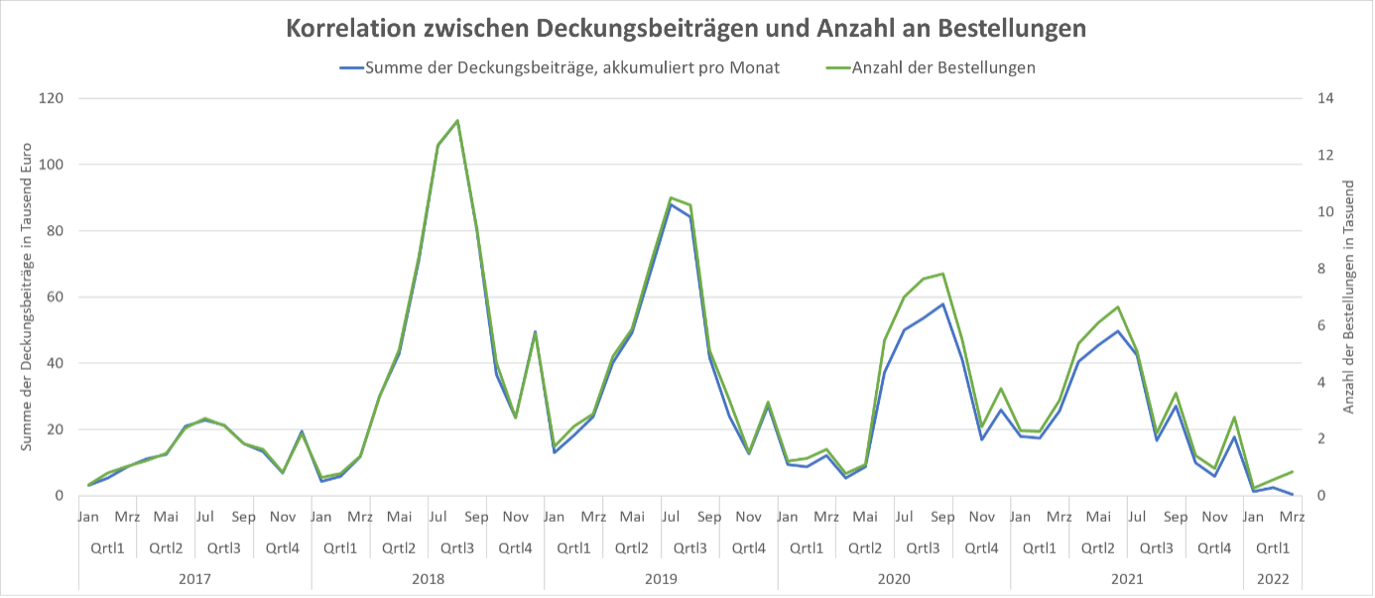
\includegraphics[width=10cm]{graphics/chart}
 	\end{center}
	\caption{Korrelation zwischen monatlichen Umsätzen und Anzahl an monatlichen Bestellungen}\label{fig:chart}
\end{figure}

\subsection{Tabellen}
\begin{table}[h]
\centering
\label{tab:sizeSearchSpace}
 \begin{tabular}{r|r|r}
      m&s&search space size\\
      \hline
      4&1&64\\
      &2&4096\\
      &3&262,144\\
      &4&16,777,216\\
      &5&1,073,741,824\\
      7&1&262144\\
      &2&16777216\\
      &3&68,719,476,736\\
      &4&2.81E+14\\
      &5&1.15E+18\\
\end{tabular}
\caption{Beispiel Tabelle}
\end{table}

\subsection{Weitere Anhänge}

\printbibliography[heading=bibintoc]  
%!TEX root = ../master.tex


\section*{Eigenständigkeitserklärung} 
\thispagestyle{empty}

\bigskip

Hiermit versichere ich,

•	dass die Arbeit, bzw. bei einer Gruppenarbeit mein entsprechend gekennzeichneter Teil, selbstständig verfasst wurde, \\[0.5cm]
•	dass keine anderen als die angegebenen Quellen benutzt und alle wörtlich oder sinn-gemäß aus anderen Werken übernommenen Aussagen als solche gekennzeichnet wurden,\\[0.5cm]
•	dass keine anderen als die angegebenen Hilfsmittel verwendet wurden,\\[0.5cm]
•	dass die eingereichte Arbeit weder vollständig noch in wesentlichen Teilen Gegenstand eines anderen Prüfungsverfahrens war und\\[0.5cm]
•	dass die Arbeit weder vollständig noch in Teilen bereits veröffentlicht wurde.\\[2cm]


Stuttgart, den\\ 

Unterschrift

%!TEX root = ../master.tex

\section*{Erklärung zur Verwendung von Künstlicher Intelligenz}

\thispagestyle{empty}
\bigskip
Im Rahmen der Erstellung der Arbeit wurden die folgenden KI-Werkzeuge wie folgt genutzt:

% Beispiele für die Verwendung von KI-Werkzeugen, diese können natürlich angepasst werden

\begin{table}[ht]
  \centering
  {\small 
    \tolerance=10000
    \emergencystretch=100mm
    \begin{tabular}{p{3cm}p{3cm}p{3cm}p{5cm}}
      \hline
      Tooltyp & Toolbezeichnung & Einsatzzweck & Prompt \\
      \hline
      LLM &
      ChatGPT auf Basis von GPT-4 &
      Ideengenerierung &
      Welche Inhalte würdest Du zum Thema Künstliche Intelligenz für die Automatisierung der Seminararbeitserstellung behandeln? \\ 
      \hline
      LLM &
      Mixtral 8x7B &
      Strukturierungshilfe &
      Wie könnte man die Systemarchitektur eines Chatbot-Systems strukturieren? \\ 
      \hline
      Bildgenerator &
      DALL-E 3&
      Visualisierung &
      Erstelle ein Bild, das die Funktionsweise eines Chatbots darstellt. \\
      \hline
    \end{tabular}
  }
\end{table}



\end{document}
% ----------------------------------------------------------
% Ende
% ----------------------------------------------------------
